Bedąc uzbrojonym~w~informacje wymienione we wcześniejszych rozdziałach można ułożyć model działania programu będącego celem tej pracy. Aby to jednak było możliwe należy wybrać najważniejsze informacje o maszynie, sytemie plików i odpowiednie strategie ich użycia.

\section{Charakterystyka typowych zmian~w~systemie plików podczas ataku ransomware}
\label{sec:charak}
Z informacji wymienionych~w~\hyperref[sec:monitorowanie]{Historia i ewolucja ataków typu ransomware} oraz~w~sekcji
\hyperref[sec:techniques]{Istniejące techniki wykrywania i obrony przed ransomware} można wyłuskać kilka punktów interakcji, które aktywują skan jedną~z~ metod przedstawionych~w~\hyperref[sec:techniques]{Istniejące techniki wykrywania i obrony przed ransomware}. Na potrzeby pracy proponuję: 
\begin{enumerate}
    \item przekroczenie obranej i dostatecznie wysokiej granicy wykonywanych operacji~w~ścieżce,
    \item duża ilość usuniętych a potem dodanych po sobie plików~w~obranym oknie czasowym (sugerująca zmianę nazw),
    \item powstanie plików zawierających~w~sobie słowa \enquote{README}, \enquote{LOG}, \enquote{ENCRYPTED},
    \item rutynowy skan~w~ustalonym przedziale czasowym.
\end{enumerate}
Pierwszy i drugi punkt będzie wymagał od administratora dostosowania współczynników liczbowych i tym samym dokonania korekty na własną rękę. Powodem tej konfiguracji jest indywidualna natura ruchu na danej maszynie. Na niektórych ruch będzie większy niż na innych co jest warte wzięcia pod uwagę. Punkt trzeci mimo, że jest wskaźnikiem na pierwszy rzut oka prymitywnym, jest usprawiedliwony zachowaniem dwóch najbardziej niebezpiecznych RaaS, wymienionych~w~sekcji \hyperref[sec:monitorowanie]{Historia i ewolucja ataków typu ransomware}. Rutynowy skan jest~w~dużej mierze ostateczną metodą która zostanie wykorzystana kiedy wszystkie inne zawiodą. Sama operacja skanowania będzie oparata na jednej lub kilku~z~metodach opisanych~w~sekcji \hyperref[sec:metody]{Metody analizy statystyk systemu plików}.
%%%%%%%%%%%%%%%%%%%%%%%%%%%%%%%%%%%%%%%%%%%%%%%%
\newpage
\section{Wybór odpowiednich statystyk i metryk do analizy}
\label{sec:wybor}
Aby móc przeanalizować ruch na wycześniej wymienione sposoby potrzebne będą informacje o:
% enumerate here 
\begin{itemize}
    \item czasie wystąpienia operacji~w~celu ustaleni ramki czasowej~w~której się zdarzyły,
    \item plikach zmodyfikowanach~w~ramach operacji,
    \item rodzaju operacji oraz plik wykonywalny który był jej źródłem,
    \item wywołaniu systemowym użytym~w~operacji.
\end{itemize}
Aby dokonać rzetelnego raportu dla administratora~w~moim przeczuciu należy także zawrzeć użytkownika oraz grupę będącą źródłem zaobserwowanej operacji. 
Zawarcie~w~tych statystykach nazwy wywołania systemowego ma znaczenie dla sprecyzowania jaka operacja \emph{naprawdę} została dokonana \cite{kernel}. Dany jest przykład użycia aplikacji \texttt{Visual Studio Code}: 
\begin{lstlisting}[language=bash,
    backgroundcolor=\color{EEGold!5!white},
    caption={Przykładowo używając \texttt{Visual Studio Code} niektóre operacje mogą
    sprawiać pozory, że na pliku wywołano polecenie \texttt{code} bez wiedzy co dokładnie zaszło podczas działania programu.},
    label={lst:helloC}]
    $ pidof code
    9551
    $ strace -p 9551
    strace: Process 9551 attached
    restart_syscall(<... resuming interrupted read ...>
    ) = 0
    futex(0x7ffcab93e008, FUTEX_WAKE_PRIVATE, 1) = 0
    lseek(26, 0, SEEK_SET)                  = 0
    read(26, "296974470 53709 24257 29420 0 82"..., 4095) = 38
\end{lstlisting}
W listingu wyżej można wydedukować na podstawie wiedzy o tym, że \texttt{Visual Studio Code} jest edytorem tekstowym, że otwarto plik~z~blokadą wykluczającą, wskaźnik~w~nim został przesunięty do miejsca zerowego dla pliku o deskryptorze numer dwadzieścia sześć oraz odczytano 4095 znaków od tamtego miejsca. Reasumując - odczytano plik do edycji i zablokowano do niego dostęp innym procesom.
\begin{figure}[H]
    \centering
    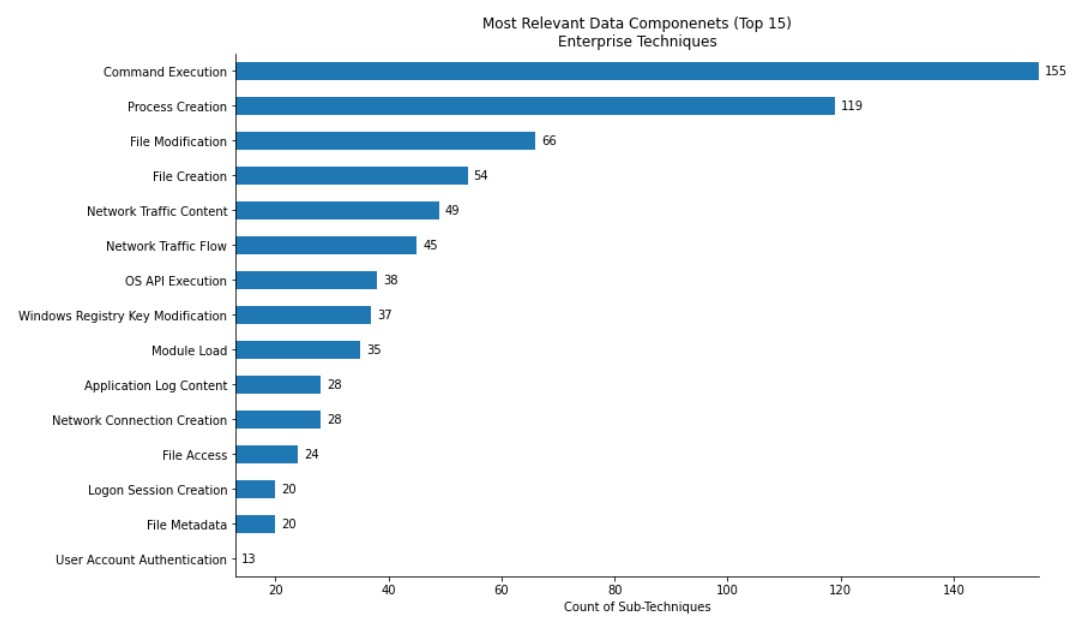
\includegraphics[width=0.75\linewidth]{rysunki/relevant_data_components.jpg}
    \caption{Najbardziej wartościowe źródła danych o ataku wg. MITRE\protect\footnotemark .}
    \label{fig:enter-label}
\end{figure}
\footnotetext{\url{https://github.com/mitre-attack/attack-datasources/blob/main/docs/images/relevant_data_components.jpg}}
%%%%%%%%%%%%%%%%%%%%%%%%%%%%%%%%%%%%%%%%%%%%%%%%
\section{Potencjalne wyzwania i ograniczenia metody}
Do najciekawszych wyzwań zaproponowanego rozwiązania należą zarówno uniwersalne aspekty techniczne jak i związane~z~doborem dystrybucji i wersji jądra systemowego Linux. Rozwiązanie wykrywające operacje musi być dostatecznie rzetelne i~w~powszechnym użyciu.~W~innym wypadku kontrola systemu będzie zwyczajnie pełna luk, które same~w~sobie będą trudne do wykrycia. Efektem złego doboru roziwązania technicznego dla funckjonalności wykrywającej operacje na systemie plików może być utrata wsparcia deweloperskiego dla głównej wersji jądra systemu.
\newline
Największym wyzwaniem od strony technicznej jest utworzenie oprogramowania, którego logika wykrywania operacji na bierząco, nie będzie prowadziła do wysokiego zużycia zasobów. Zbieranie dużej ilości informacji~z~pokaźnego ciągu operacji bez wątpliwości będzie mieć wpływ na zużycie zasobów systemowych. Nie ma możliwości całkowitej eliminacji tego wpływu, można jednak podjąć kroki~w~doborze technologii~w~celu zniwelowania go. 
\newline
Mimo iż postanowiłem wybrać przypadki aktywacji funkcji skanowania ścieżki, która zazębia~z~powszechnymi scenariuszami ataku, istnieje możliwość niewystarczającego pokrycia przypadków. 
\newline
Trzeba też zaznaczyć, że dla plików skompresowanych badanie entropii ich treści może wskazywać na błędną klasyfikację~w~ramach metody przedstawionej~w~sekcji \hyperref[sec:entropia] {Analiza entropii pliku}. Nie jest to szczególnie duży problem ze względu na to, że metoda charakteryzuje się wysoką dokładnością dla plików o wielkości większej niż 32 bajty, wielkości, której przekroczenie nie jest ciężkim wyzwaniem dla plików skompresowanych. 
\newline
Metoda zaprezentowana~w~rozdziale \hyperref[sec:binaries] {Analiza podobieństwa pliku wykonywalnego} także nie jest jednoznaczną metodą wykrycia zagrożenia. Cytując abstrakt pracy \foreignquote{english}{A Framework for Analyzing Ransomware using
Machine Learning}~\cite{8628743} : \foreignquote{english}{Experimental results reported the performance
i.e. the detection accuracy of ransomware samples which varied
from 76\% to 97\% based on the ML technique used [...]}, można się spodziewać fałszywego stwierdzenia obecności ransomware~w~podobnym,~a~może i nawet rozleglejszym przedziale dokładności. 
\newline
Analizując te braki trzeba mieć na uwadze, że projektowany program ma być jednym z wielu narzędzi dla administratora ale nie ma zwalniać go z obowiązku rzetelnego analizowania potencjalnych zagrożeń na systemie. Nie ma on też być rozwiązaniem typu \enquote{wszystko w jednym}. Jego celem jest mitygacja kosztów ataku poprzez poinformowanie administratora o możliwości ataku.
